%!TEX program = xelatex
\documentclass[a4paper,12pt, centering]{ctexart}
\usepackage[colorlinks=true,linkcolor=blue,urlcolor=black,bookmarksopen=true]{hyperref}
\usepackage{bookmark}

\usepackage{geometry}
\geometry{left=2.5cm,right=2cm,top=2.5cm,bottom=2.5cm}

\usepackage{graphicx}
\graphicspath{ {./assets/} }

% Add support for font config.
\usepackage{fontspec}

% Add support for code snippet.
\usepackage{listings}

% Add color support for code snippet.
\usepackage{xcolor}

% Set Fira Code as the font for code snippet
\setmonofont[
  Contextuals={Alternate}
]{Fira Code}

% Color settings for code snippet.
\definecolor{codegreen}{rgb}{0,0.6,0}
\definecolor{codegray}{rgb}{0.5,0.5,0.5}
\definecolor{codepurple}{rgb}{0.58,0,0.82}
\lstdefinestyle{mystyle}{
    commentstyle=\color{codegreen},
    keywordstyle=\color{magenta},
    numberstyle=\tiny\color{codegray},
    stringstyle=\color{codepurple},
    basicstyle=\ttfamily,
    breakatwhitespace=false,
    breaklines=true,
    captionpos=b,
    keepspaces=true,
    numbers=left,
    numbersep=5pt,
    showspaces=false,
    showstringspaces=false,
    showtabs=false,
    tabsize=2
}
\lstset{style=mystyle}

\title{基于Angular和NestJS的动漫平台评论网站系统}
\author{佘嘉洛\footnote{电子邮件: shejialuo@stu.xidian.edu.cn,
     学号:21031211515}\\[2ex] 计算机科学与技术学院 软件工程专业
     \\[2ex] Made By \LaTeX}
\date{2021年12月25日}

\begin{document}
  \
  \vspace{6cm}
  \begingroup
  \let\newpage\relax
  \maketitle
  \thispagestyle{empty}
  \endgroup

  \newpage

  \setcounter{page}{1}

  \section*{1. 项目简介}

  本项目拟实现一个全栈的动漫平台评论网站系统。实现如下的功能:

  \begin{itemize}
    \item 用户注册功能
          \begin{itemize}
            \item 前端表单验证用户两次输入的密码是否一致。
            \item 后端验证用户注册的用户名是否重名,前端需防抖。
            \item 发送邮件验证,用户需输入正确的验证码才能注册。
          \end{itemize}
    \item 用户登录功能
          \begin{itemize}
            \item 前端用户为登录时,用户使用用户名和密码登陆
            \item 第一次登录,后端验证利用JWT生成token,前端
                  通过Response对象获取token,存储在
                  LocalStorage中,不使用cookie,避免CSRF。
            \item 登录后,在token有效期内,前端用户无需再次登陆。
          \end{itemize}
    \item 用户评论功能
  \end{itemize}

  \section*{2. 技术栈选取}

  本项目采用前后端分离开发的方式进行。

  \subsection*{2.1 前端}

  本项目前端采取Angular框架进行开发。Angular框架是由是一个基于TypeScript的开源
  Web应用框架由Google的Angular团队以及社区共同领导。同时,本项目采用Angular官方
  的基于Material Design的样式库Angular Material作为组件开发库:

  \begin{itemize}
    \item Angular Version: 13.0.3
    \item Angular Material Version: 13.0.1
  \end{itemize}

  \subsection*{2.2 数据库}

  本项目使用非关系型数据库MongoDB作为数据库,采用Mongoose作为
  数据库处理高层语言。

  \subsection*{2.3 后端}

  本项目使用NestJS作为后端开发。

  \section*{3. 项目架构设计}

  本节阐述本项目的架构设计,整体架构设计如图1所示。

  \begin{figure}[h]
    \centering
    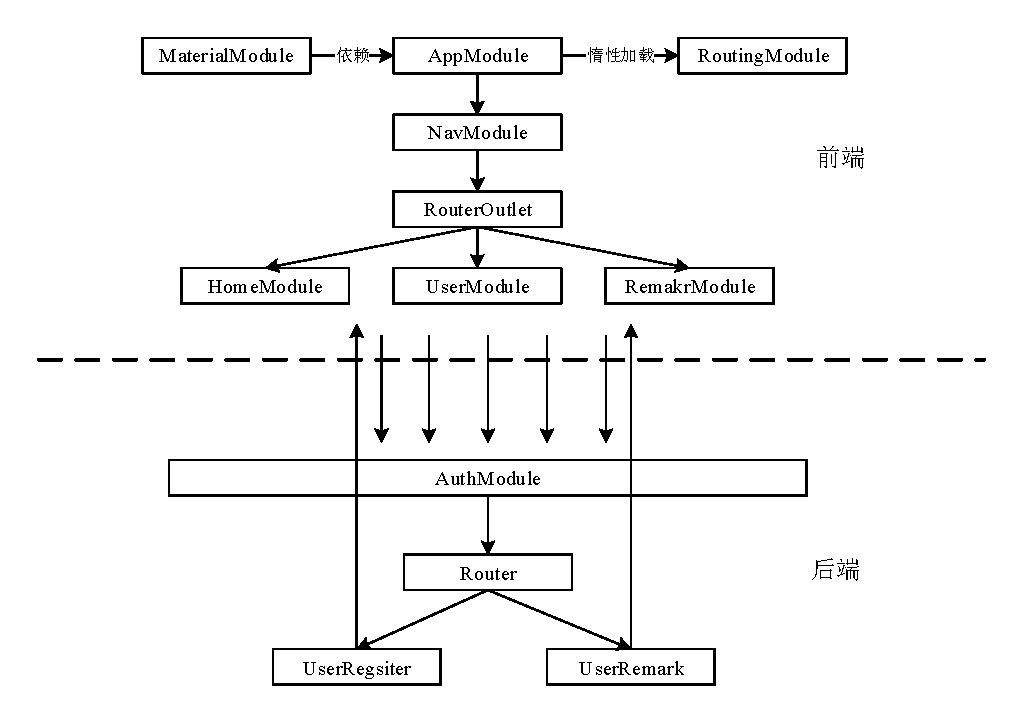
\includegraphics[width=\textwidth]{1.pdf}
    \caption{项目整体架构示意图}
  \end{figure}

  \section*{4. 关键技术解决}

  本节阐述在开发过程中解决的关键技术问题

  \subsection*{4.1 数据库设计}

  由于采用非关系性数据库且本项目业务逻辑较简单,本项目的数据库
  设计比较简单,本项目设置了两个类\verb|User|, \verb|Remark|
  即完成了数据库设计,如下所示:

  \begin{lstlisting}[language=java, caption=数据库设计]
  @Schema()
  export class User {
    @Prop({ required: true })
    userName: string;

    @Prop({ required: true })
    userPassword: string;

    @Prop({ required: true })
    userEmail: string;
  }
  @Schema()
  export class Remark {
    @Prop({ required: true })
    userName: string;
    
    @Prop({ required: true })
    userRemark: string;
  }
}
  \end{lstlisting}

  \subsection*{4.2 注册表单实现}

  表单的实现是一个关键,主要实现的还是验证的功能。前端的表单验证分为
  了两个类型:

  \begin{itemize}
    \item 前端直接验证
    \item 后端验证
  \end{itemize}

  本项目对于这两种类型的验证均涉及到了。首先是前端验证用户输入的密码
  以及确认密码是否一致,本项目通过Angular框架自带的响应式表单很容易
  地实现了前端直接验证。整个表单通过\verb|FormGroup|控制,表单的
  字段通过\verb|FormControl|控制。通过响应式表单,由函数控制表单,
  而不是在\verb|HTML|模板中使用模板变量控制,从而实现了模板与控制器
  的解耦。

  \begin{figure}[h]
    \centering
    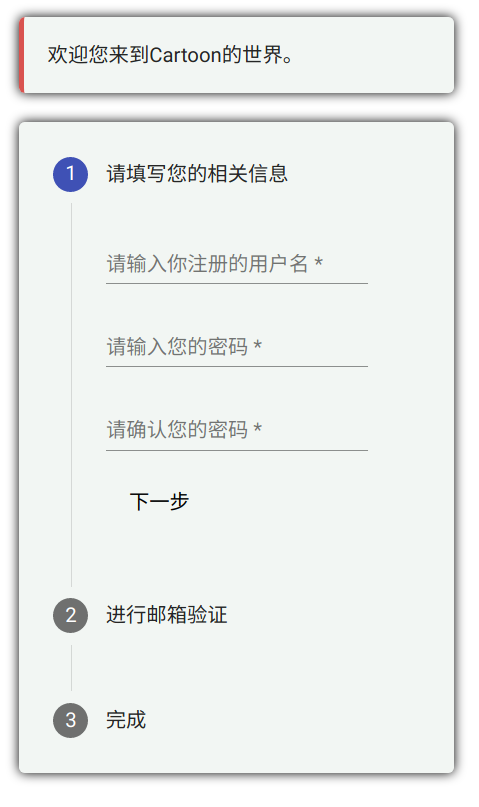
\includegraphics{1.png}
    \caption{前端表单步进器设计}
  \end{figure}

  \subsubsection*{4.2.1 用户名重名验证}
  由图2可以看出,对于第一个步骤“请填写您的相关信息”,本文通过建立一个
  关键的\verb|FormGroup|类\verb|passwordFormGroup|控制,同时
  建立三个\verb|FormControl|,如下所示:

  \begin{lstlisting}[language=java, caption=响应式表单代码]
    this.passwordFormGroup = this.formBuilder.group({
      userName: ['', [Validators.required, Validators.minLength(6)], this.userNameValidators],
      userPrePassword: ['', [Validators.required, Validators.minLength(6)]],
      userPostPassword: ['', [Validators.required, this.passwordValidators]],
    });
  \end{lstlisting}

  可以看出,对于注册的用户名,本项目使用内置的同步验证器表明用户必须输入,
  且至少需要6位。同时,本项目定义了一个自定义的异步验证器用于查询用户名
  是否重名。显然,此步需要进行防抖的操作。

  \begin{lstlisting}[language=java, caption=验证用户名是否重名]
    userNameValidators: AsyncValidatorFn = (control: AbstractControl) => {
      return control.valueChanges.pipe(
        debounceTime(1000),
        distinctUntilChanged(),
        switchMap(() => {
          return this.userService.checkName(control.value);
        }),
        map(result => result ? {isSame: true}: null),
        first(),
      )
    }
  \end{lstlisting}
  
  从上述代码可以看出,每当\verb|FormControl|的值改变时,将会进行一系列
  的判断。首先时用户在1s内没有执行输入的操作,且输入的值没有发生改变,往
  后端发送请求,查询数据库是否存在同名的用户名。

  \begin{figure}[h]
    \centering
    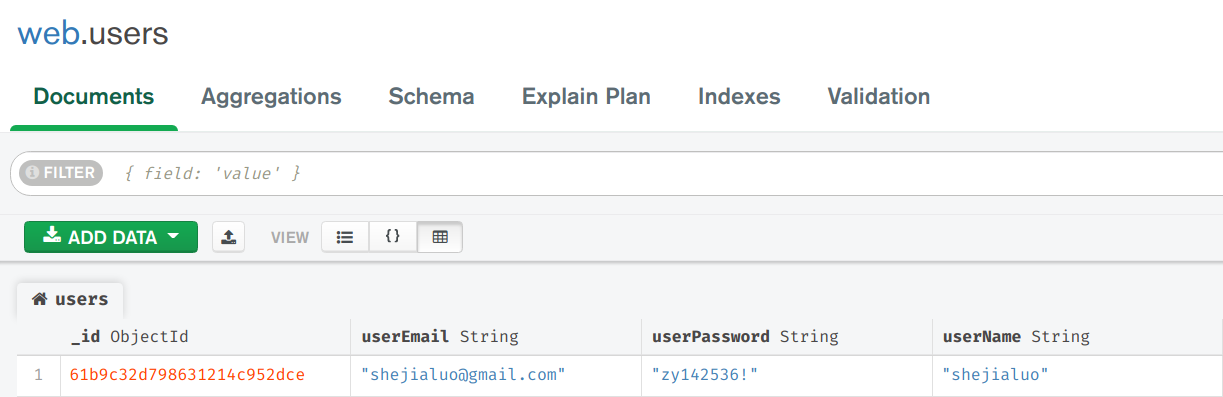
\includegraphics[width=\textwidth]{2.png}
    \caption{MongoDB数据库展示}
  \end{figure}

  如图3所示,此时系统已经注册了一位用户名为\verb|shejialuo|的用户。
  此时,如图4所示,在注册表单输入用户名\verb|shejialuo|将会提示红字
  用户名已经重名请修改。

  \begin{figure}[h]
    \centering
    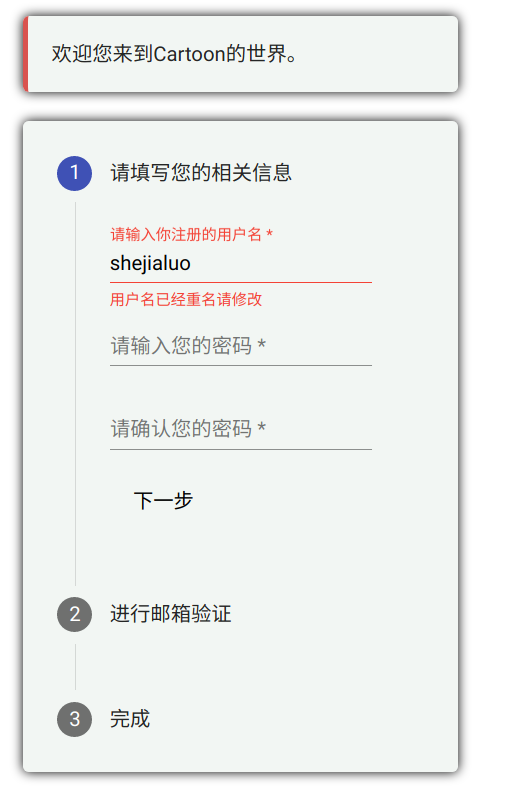
\includegraphics{3.png}
    \caption{用户名重名示意图}
  \end{figure}

  \subsubsection*{4.2.2 验证输入密码一致}

  4.2.1节中阐述的是异步验证,也就是通过后端请求的数据返回前端做表单验证,
  本节将阐述同步验证。其实现的思路比较简单,就是比较值,此处不赘述,
  如图5所示。

  \begin{figure}[h]
    \centering
    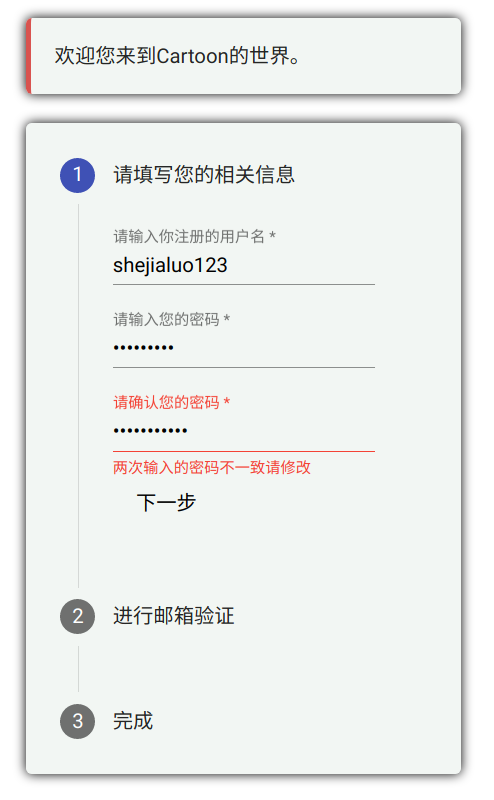
\includegraphics{4.png}
    \caption{用户输入密码不一致示意图}
  \end{figure}

  \subsubsection*{4.2.3 邮箱验证}

  邮箱验证实现的思路是比较简单的,对于前端而言,首先要对邮件的格式做验证。
  后发送请求至后端。后端通过产生4位数的随机码,通过SMTP发送即可。
  为了维持状态,维持一个\verb|MAP<emailAddress, checkCode>|即可。

  \subsection*{4.3 登录}

  本小节阐述本项目如何实现登录功能,本项目通过JWT实现验证。其
  基本的思想是用户通过输入用户名和密码登录,后端进行验证,通过JWT返回
  token。前端接收到后端的Response,提取出token,将其保存到
  LocalStorage中,后用户在有效期内,可以直接免密登录。

  \subsubsection*{4.3.1 后端JWT生成}

  由于NestJS框架提供了内置的JWT模块,可以直接通过依赖注入实现功能。故
  对于用户使用用户名和密码登录的情况,本项目查询数据库,如果满足,则发送
  JWT Token提供给前端。

  \begin{lstlisting}[language=java, caption=后端JWT生成并传递给前端]
    @Post('login')
    async login(@Res({passthrough: true}) 
          response: FastifyReply ,
          @Body() loginDto: LoginDto) {
      let loginSuccess = await this.authService.userLogin(loginDto);
  
      if(!loginSuccess) {
        response.send({success: false});
      } 
      else {
        const userId = loginDto.userName;
        const payload = {userId: userId};
        const token = this.jwtService.sign(payload);
        response.send({
          success: true,
          jwtToken: token});
      }
    }
  \end{lstlisting}

  \subsubsection*{4.3.2 前端保存Token}

  前端需要把后端发送的Token保存到LocalStorage中,这一点相对容易比较
  实现。此处就不赘述了。

  \subsubsection*{4.3.3 前端实现Token注入Header}

  由于本项目将Token保存在LocalStorage中,不像cookie在每次进行HTTP
  通信时,会自动将其注入Header。因此,在每一次进行HTTP通信时,都需要把
  Token注入Header中,以便于用于后端的验证。显然,这一步最好透明化,
  Angular框架提供了HTTP Interceptor机制可以透明地实现这一功能:

  \begin{lstlisting}[language=java, caption=前端Header自动注入Token]
    export class AuthInterceptor implements HttpInterceptor {
    intercept(req: HttpRequest<any>,
              next: HttpHandler): Observable<HttpEvent<any>> {

      const idToken = localStorage.getItem("id_token");

      if (idToken) {
        const cloned = req.clone({
        headers: req.headers.set("Authorization",
                  idToken)
        });

        return next.handle(cloned);
      }
      else {
        return next.handle(req);
      }
    }
}
  \end{lstlisting}

  通过如上的操作既可以透明实现Token注入Header。

  \section*{5. 总结}

  麻雀虽小,五脏俱全。

\end{document}

